\documentclass[conference]{IEEEtran}
\IEEEoverridecommandlockouts
\usepackage{cite}
\usepackage{amsmath,amssymb,amsfonts}
\usepackage{graphicx}
\usepackage{textcomp}
\usepackage[table]{xcolor}
\definecolor{diagcolor}{RGB}{29,158,117}
\definecolor{offdiagcolor}{RGB}{216,90,48}
\pagestyle{plain}

\begin{document}

\title{Metadata-Guided Cross-Attention Fusion for Multimodal Skin Lesion Classification: A Leakage-Audited, Cross-Dataset Validated Approach}

\author{
\IEEEauthorblockN{Md. Naeem Sarker\textsuperscript{1}, Fatema Bosri\textsuperscript{2}, Aninda Roy Dhruba\textsuperscript{3}}
\IEEEauthorblockA{\textsuperscript{1,2,3}Department of Computer Science \& Engineering\\
Northern University Bangladesh, Dhaka, Bangladesh\\
Email: naeemsarker2003.dev@gmail.com, fatemabosriborsha@gmail.com, anindaroydhruv@gmail.com}
}

\maketitle

\begin{abstract}
Skin lesion classification systems often report inflated performance due to data leakage, image-wise (non-patient-wise) splitting, and evaluation on a single dataset. We present a multimodal fusion architecture that combines dermoscopic/clinical images with structured patient metadata via cross-attention, where metadata queries guide the model's attention over spatial image features. Our pipeline includes a systematic leakage audit (22 columns excluded across 4 datasets, each backed by statistical evidence), patient-wise splitting, and evaluation on a held-out test set touched exactly once. On PAD-UFES-20 (6-class, macro-F1), our cross-attention fusion model achieves 0.6977 test macro-F1, significantly outperforming late fusion and single-modality baselines (all $p \leq 0.002$). Cross-dataset evaluation on HAM10000 and ISIC archives, bootstrap significance testing, and Fitzpatrick skin-tone fairness analysis further validate the model's generalization and equity properties. We additionally report extended ablations (backbone comparison, dataset expansion, ensemble, joint three-way fusion) under a pre-registered decision protocol, providing a transparent, reproducible account of what improved performance and what did not. Our results demonstrate that methodological rigor and honest reporting are as important as raw accuracy for clinically deployable dermatology AI.
\end{abstract}

\begin{IEEEkeywords}
multimodal fusion, cross-attention, skin lesion classification, data leakage, cross-dataset generalization, fairness
\end{IEEEkeywords}

\section{Introduction}
Skin cancer and other dermatological conditions are among the most prevalent diseases worldwide, and early, accurate diagnosis substantially improves patient outcomes, particularly since visual inspection remains the first and most accessible point of clinical contact in many healthcare settings. Automated screening tools deployed alongside, rather than in place of, dermatologist judgment therefore have direct practical value, especially where specialist access is limited. Computer-aided diagnosis (CAD) systems built on deep learning achieve strong performance on dermoscopic image classification; however, most rely on image features alone, despite dermatologists routinely incorporating patient history -- age, lesion duration, itching, prior growth, anatomical site -- into their reasoning. Metadata of this kind is frequently available in public dermatology datasets but remains underused as a modeling signal.

A second, equally important limitation concerns evaluation rigor. Many reported results are obtained under conditions that inflate apparent performance: binary framing (malignant versus benign) rather than the clinically relevant multi-class problem; accuracy as the primary metric, which can mask poor performance on minority classes in imbalanced data; absence of a documented leakage audit; and evaluation confined to a single dataset, which does not test whether a model generalizes beyond the imaging conditions, patient population, and label-collection procedure of its training source.

A third, frequently overlooked limitation concerns class imbalance. Public dermatology datasets are dominated by common, low-risk classes, while clinically urgent classes such as Melanoma are severely underrepresented. Many prior works address this purely through synthetic augmentation, which adds no genuinely new diagnostic signal. We instead source additional real, biopsy-confirmed images for the weakest classes from independent public collections, and empirically isolate how much this data-level intervention contributes relative to architectural improvements.

Beyond the modeling question, a growing body of work raises concerns about equity in dermatology AI: models trained predominantly on lighter skin tones can silently underperform on darker skin tones, a risk rarely measured, let alone reported, in typical benchmark papers. A trustworthy skin lesion classifier therefore needs to be evaluated not just for accuracy, but for the integrity of its evaluation protocol and its behavior across sub-populations.

This work addresses these limitations directly, proposing a metadata-guided cross-attention fusion architecture paired with a rigorous, transparently documented evaluation protocol. Our contributions are as follows:

\begin{enumerate}
\item A cross-attention fusion architecture in which patient metadata queries spatial image tokens, avoiding the dimensional imbalance that undermines naive late-fusion approaches.
\item A systematic, statistically-grounded leakage-audit methodology, applied across four datasets, identifying and excluding twenty-two metadata columns that would otherwise allow the model to exploit post-diagnosis information.
\item A targeted, real-data class-imbalance correction for the two rarest diagnostic classes, isolated experimentally from architectural effects.
\item Cross-dataset generalization testing (PAD-UFES-20 to HAM10000) and external validation on two ISIC archives, quantifying how performance transfers beyond the training distribution.
\item Bootstrap-based statistical significance testing for cross-dataset and extended-ablation comparisons, and a Fitzpatrick skin-tone fairness analysis.
\item A pre-registered protocol for extended architecture and data ablations, reported honestly, including results that did not exceed the primary model.
\end{enumerate}

The remainder of this paper is organized as follows. Section II reviews prior machine learning and deep learning approaches to skin lesion classification. Section III describes our datasets, leakage-audit methodology, and proposed architecture. Section IV presents our experimental results, including cross-dataset generalization, fairness analysis, and extended ablations. Section V discusses the implications and limitations of our findings, and Section VI concludes with directions for future work.

\section{Related Work}

\subsection{Machine Learning-Based Approaches}
Early computer-aided diagnosis systems for skin lesions relied on handcrafted feature extraction (color histograms, texture descriptors, border irregularity measures) combined with classical classifiers. More recent tabular-only approaches use structured clinical data directly instead of hand-engineered image features. The TRACE framework applies transformer-based modeling to structured patient metadata, showing clinical fields alone carry substantial diagnostic signal without image input. However, TRACE's PAD-UFES-20 evaluation uses a 90/10 train-validation split with no held-out test set, so its reported DANET (0.625) and TRACE (0.783) macro-F1 figures are validation-style estimates, not results comparable to a true test-set score.

\subsection{Deep Learning-Based Approaches}
The dominant paradigm fine-tunes CNNs (e.g., ResNet, EfficientNet) on dermoscopic images, often without leveraging clinical metadata. More recently, vision-language approaches have entered the field: Shrestha and Palit (2026) combine MedCLIP-derived image-text embeddings with patient metadata through early and attention-based fusion on a curated ISIC 2024 subset, reporting 96\% accuracy and an AUROC of 0.987. This is a binary-classification, accuracy-based result and, like the tabular comparators above, not directly comparable to our multi-class macro-F1 evaluation, though it illustrates the value of combining vision-language representations with metadata.

\subsection{Multimodal Fusion Mechanisms}
A smaller body of work directly addresses multimodal image-metadata fusion mechanisms. Pacheco and Krohling's MetaBlock, from PAD-UFES-20's creators, modulates image feature channels via a metadata-conditioned gating function applied uniformly across spatial locations -- unlike this work's per-location spatial cross-attention. The same authors' earlier clinical-impact study found Squamous Cell Carcinoma and Basal Cell Carcinoma share near-identical clinical profiles and remain confused even with metadata, corroborated by our own confusion analysis (Section IV-A). Comparative studies of fusion strategies on HAM10000 independently found cross-attention (image=K/V, metadata=Q) outperforms naive concatenation and self-attention, corroborating our architectural choice.

\subsection{Fairness in Dermatology AI}
Fairness in dermatology AI has received growing attention following Daneshjou et al.'s (2022) demonstration that dermatology AI models can suffer a 27--36 percentage point drop in ROC-AUC when evaluated on the Diverse Dermatology Images dataset, particularly for darker Fitzpatrick skin types and uncommon diseases. Alipour et al. (2024) subsequently showed that this is a systemic reporting and representation gap across public dermatology datasets rather than an isolated finding. To our knowledge, no prior work combines a statistically-audited leakage methodology, cross-dataset generalization testing, bootstrap significance testing, and Fitzpatrick fairness analysis within a single, transparently reported pipeline. Table \ref{tab:litcompare} summarizes these comparisons.

\begin{table}[t]
\caption{Comparison with related work}
\label{tab:litcompare}
\centering
\scriptsize
\begin{tabular}{|p{1.3cm}|p{1.1cm}|p{1.1cm}|p{1.15cm}|p{1.15cm}|}
\hline
\textbf{Aspect} & \textbf{Our Work} & \textbf{TRACE} & \textbf{Meta- Block} & \textbf{Shrestha \& Palit} \\
\hline
Approach type & DL, multimodal & ML, tabular & DL, multimodal & DL, VLM+meta \\
\hline
Modality & Image+Meta & Metadata only & Image+Meta & Image+Meta (VLM) \\
\hline
Classes & 6 & N/D\textsuperscript{a} & N/C\textsuperscript{b} & 2 (binary) \\
\hline
Metric & Macro-F1 & Macro-F1 & Acc.\textsuperscript{c} & Accuracy \\
\hline
Held-out test & Yes & No (val-only) & N/C\textsuperscript{b} & Yes \\
\hline
Leakage audit & 22 cols. & Not reported & N/C\textsuperscript{b} & Not reported \\
\hline
Cross-dataset & Yes & No & N/C\textsuperscript{b} & No \\
\hline
Fairness & Yes & No & N/C\textsuperscript{b} & No \\
\hline
\end{tabular}
\\[2pt]
\raggedright{\scriptsize \textsuperscript{a}N/D: not documented. \textsuperscript{b}N/C: unconfirmed, source paywalled; retained for completeness. \textsuperscript{c}Secondary-source figure, unverified.}
\end{table}

\section{Methodology}

Figure \ref{fig:overview} presents an overview of our dataset preparation pipeline, from raw data sourcing through the leakage-audited, patient-wise-split processed output, before we describe each phase in detail.

\begin{figure}[t]
\centering
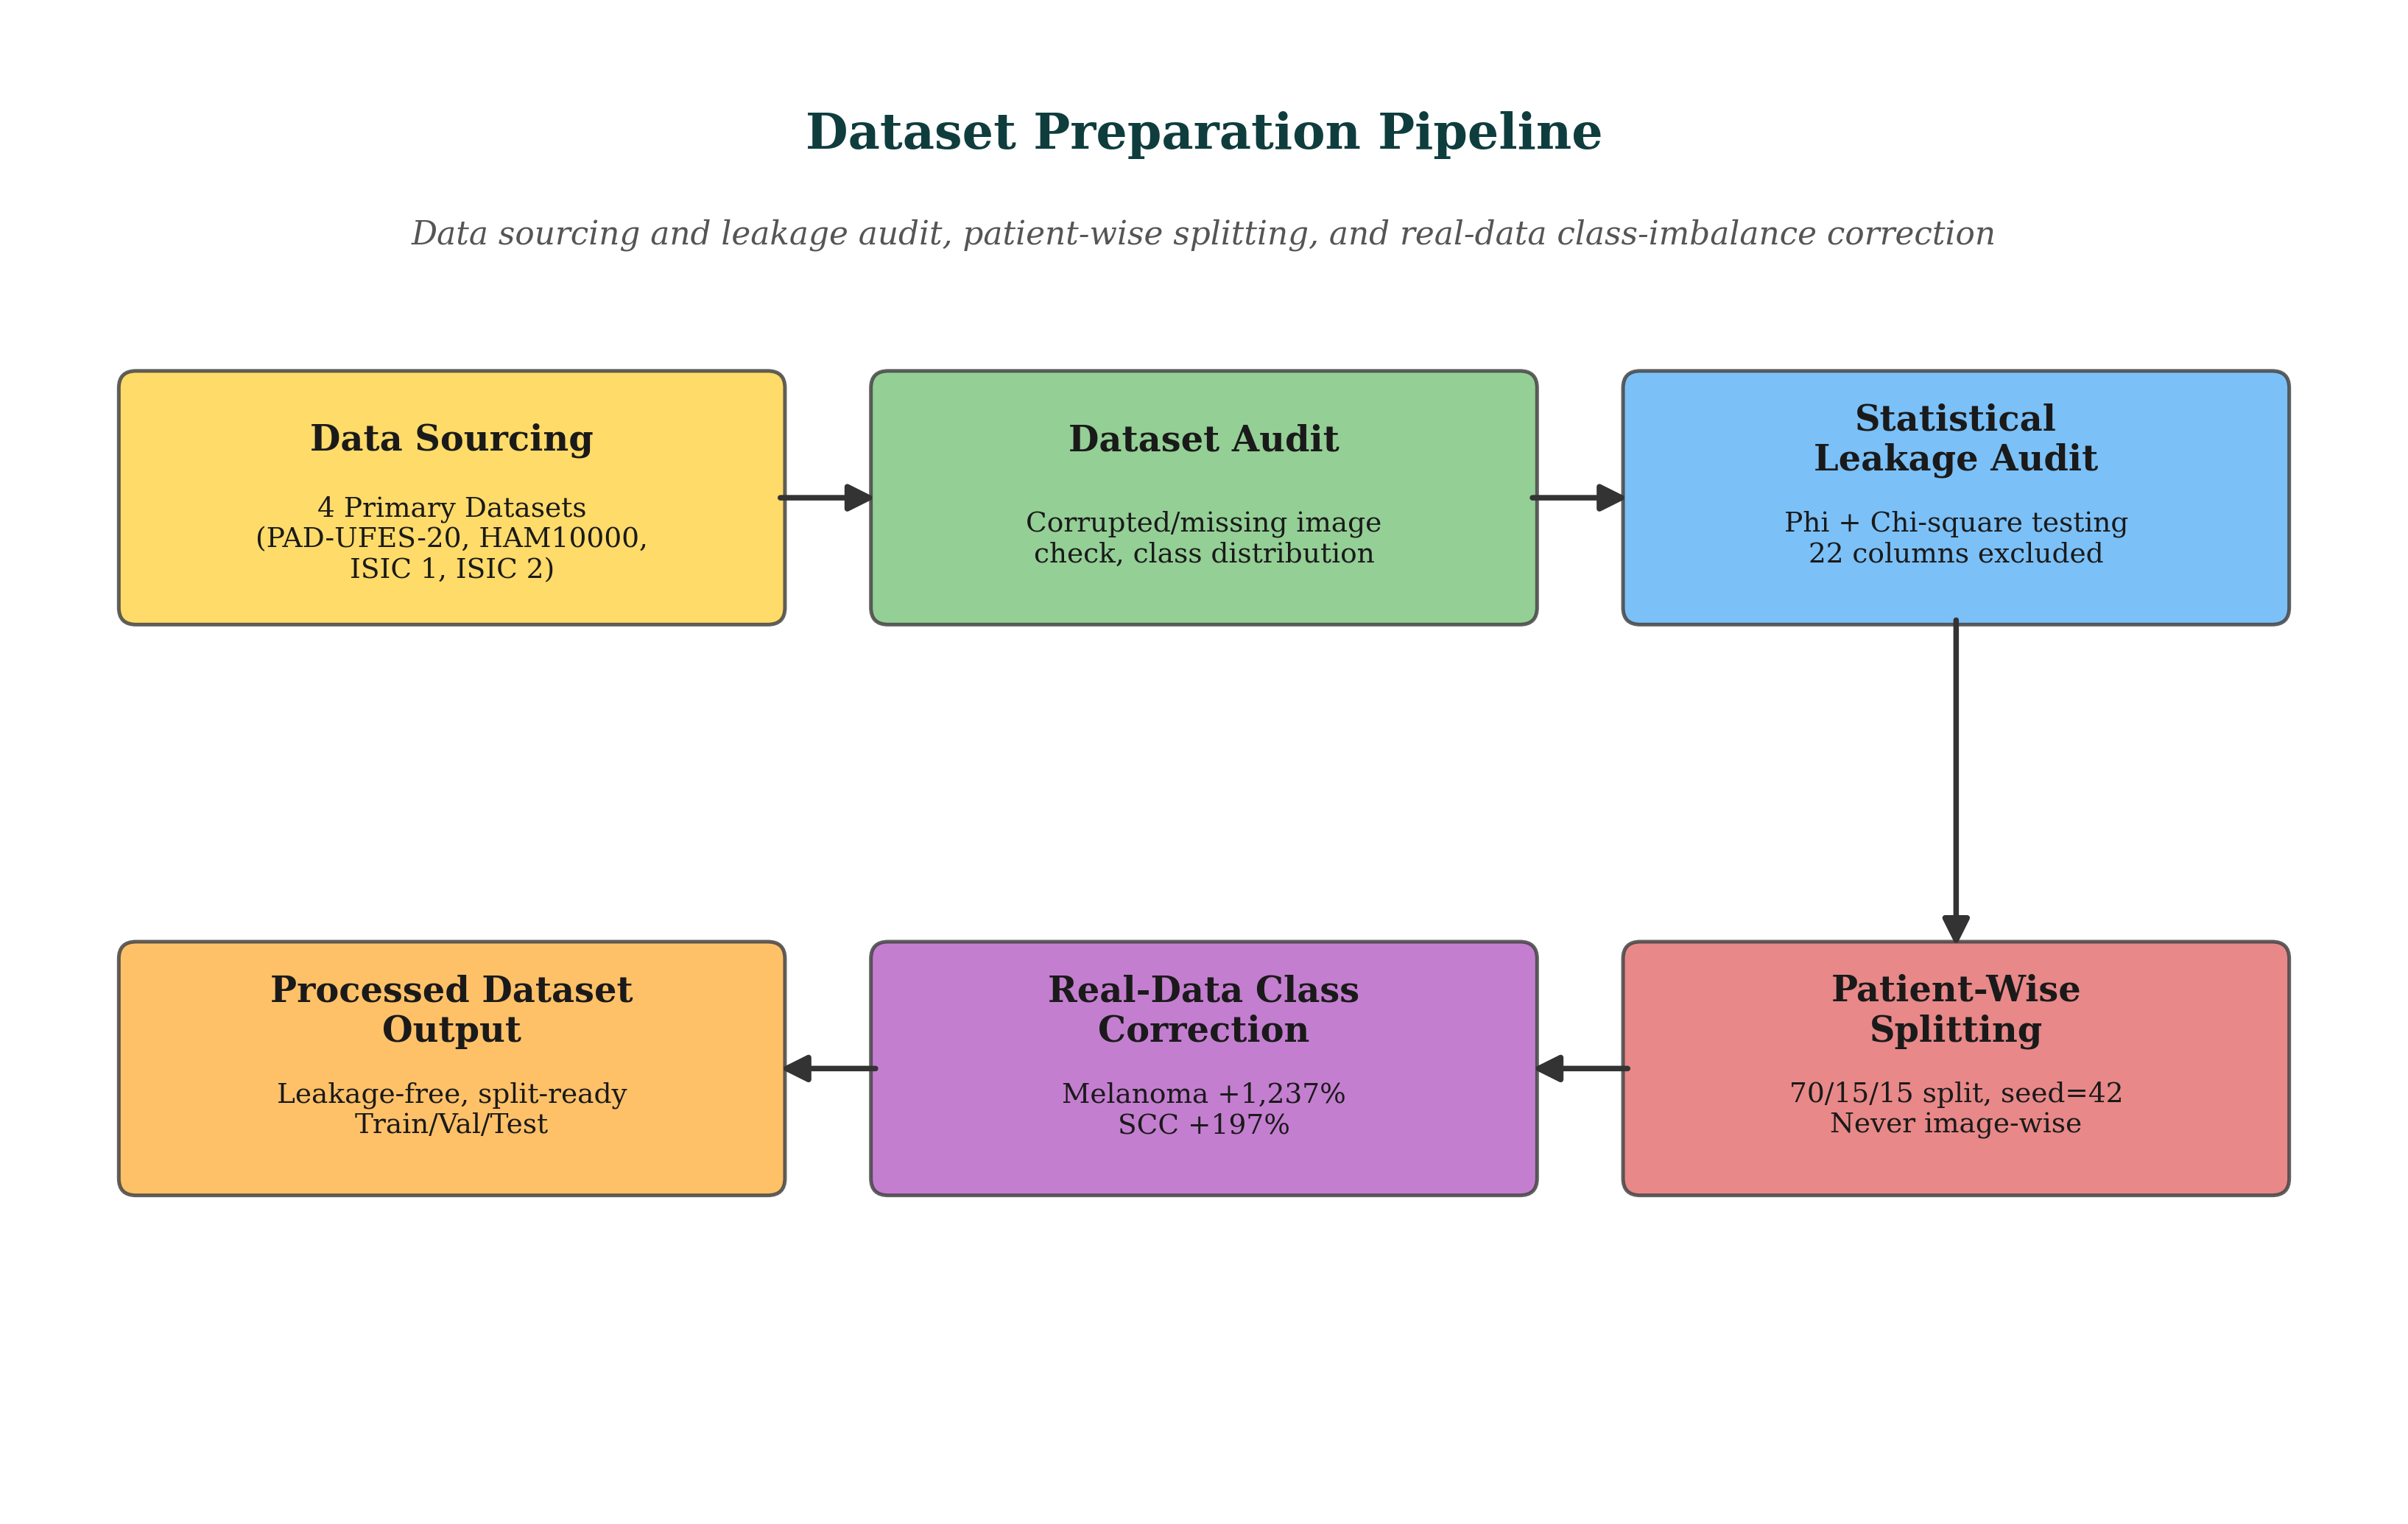
\includegraphics[width=0.85\columnwidth]{workflow_overview.pdf}
\caption{Dataset preparation pipeline: data sourcing, quality audit, statistical leakage audit, patient-wise splitting, real-data class-imbalance correction, and the resulting processed dataset.}
\label{fig:overview}
\end{figure}

\subsection{Datasets}
Table \ref{tab:datasets} summarizes the four datasets used in this study. PAD-UFES-20 (2,298 images, six diagnostic classes) serves as the primary dataset for training and final evaluation, and is the only dataset among those used that provides rich structured clinical metadata (twenty-one usable features after audit) -- a key distinguishing property of our data foundation, since it is what makes genuine image+metadata fusion possible at all. HAM10000 (10,015 images, seven classes) is used exclusively as a cross-dataset generalization target. ISIC Archive 1 (2,357 images) and ISIC Archive 2 (25,076 images) are used solely for external validation and were never included in any training set.

\begin{table}[t]
\caption{Dataset overview}
\label{tab:datasets}
\centering
\begin{tabular}{|l|c|c|c|}
\hline
\textbf{Dataset} & \textbf{Images} & \textbf{Classes} & \textbf{Role} \\
\hline
PAD-UFES-20 & 2,298 & 6 & Primary train/val/test \\
\hline
HAM10000 & 10,015 & 7 & Cross-dataset generalization \\
\hline
ISIC Archive 1 & 2,357 & 9 & External validation \\
\hline
ISIC Archive 2 & 25,076 & 9 & External validation \\
\hline
\end{tabular}
\end{table}

To address severe class imbalance in the two rarest PAD-UFES-20 categories, we incorporated biopsy-confirmed images from two external, non-overlapping public sources, expanding Melanoma from 38 to 508 images (a 1,237\% increase) and Squamous Cell Carcinoma from 135 to 401 images (a 197\% increase), as shown in Figure \ref{fig:imbalance}. Unlike synthetic augmentation, every added image is a real, independently-sourced, biopsy-confirmed case, verified to have zero patient overlap with any evaluation split. This expanded variant is used only in the later ablation experiments (Section IV-E), never in the primary reported result, preserving the integrity of our locked headline evaluation.

\begin{figure}[t]
\centering
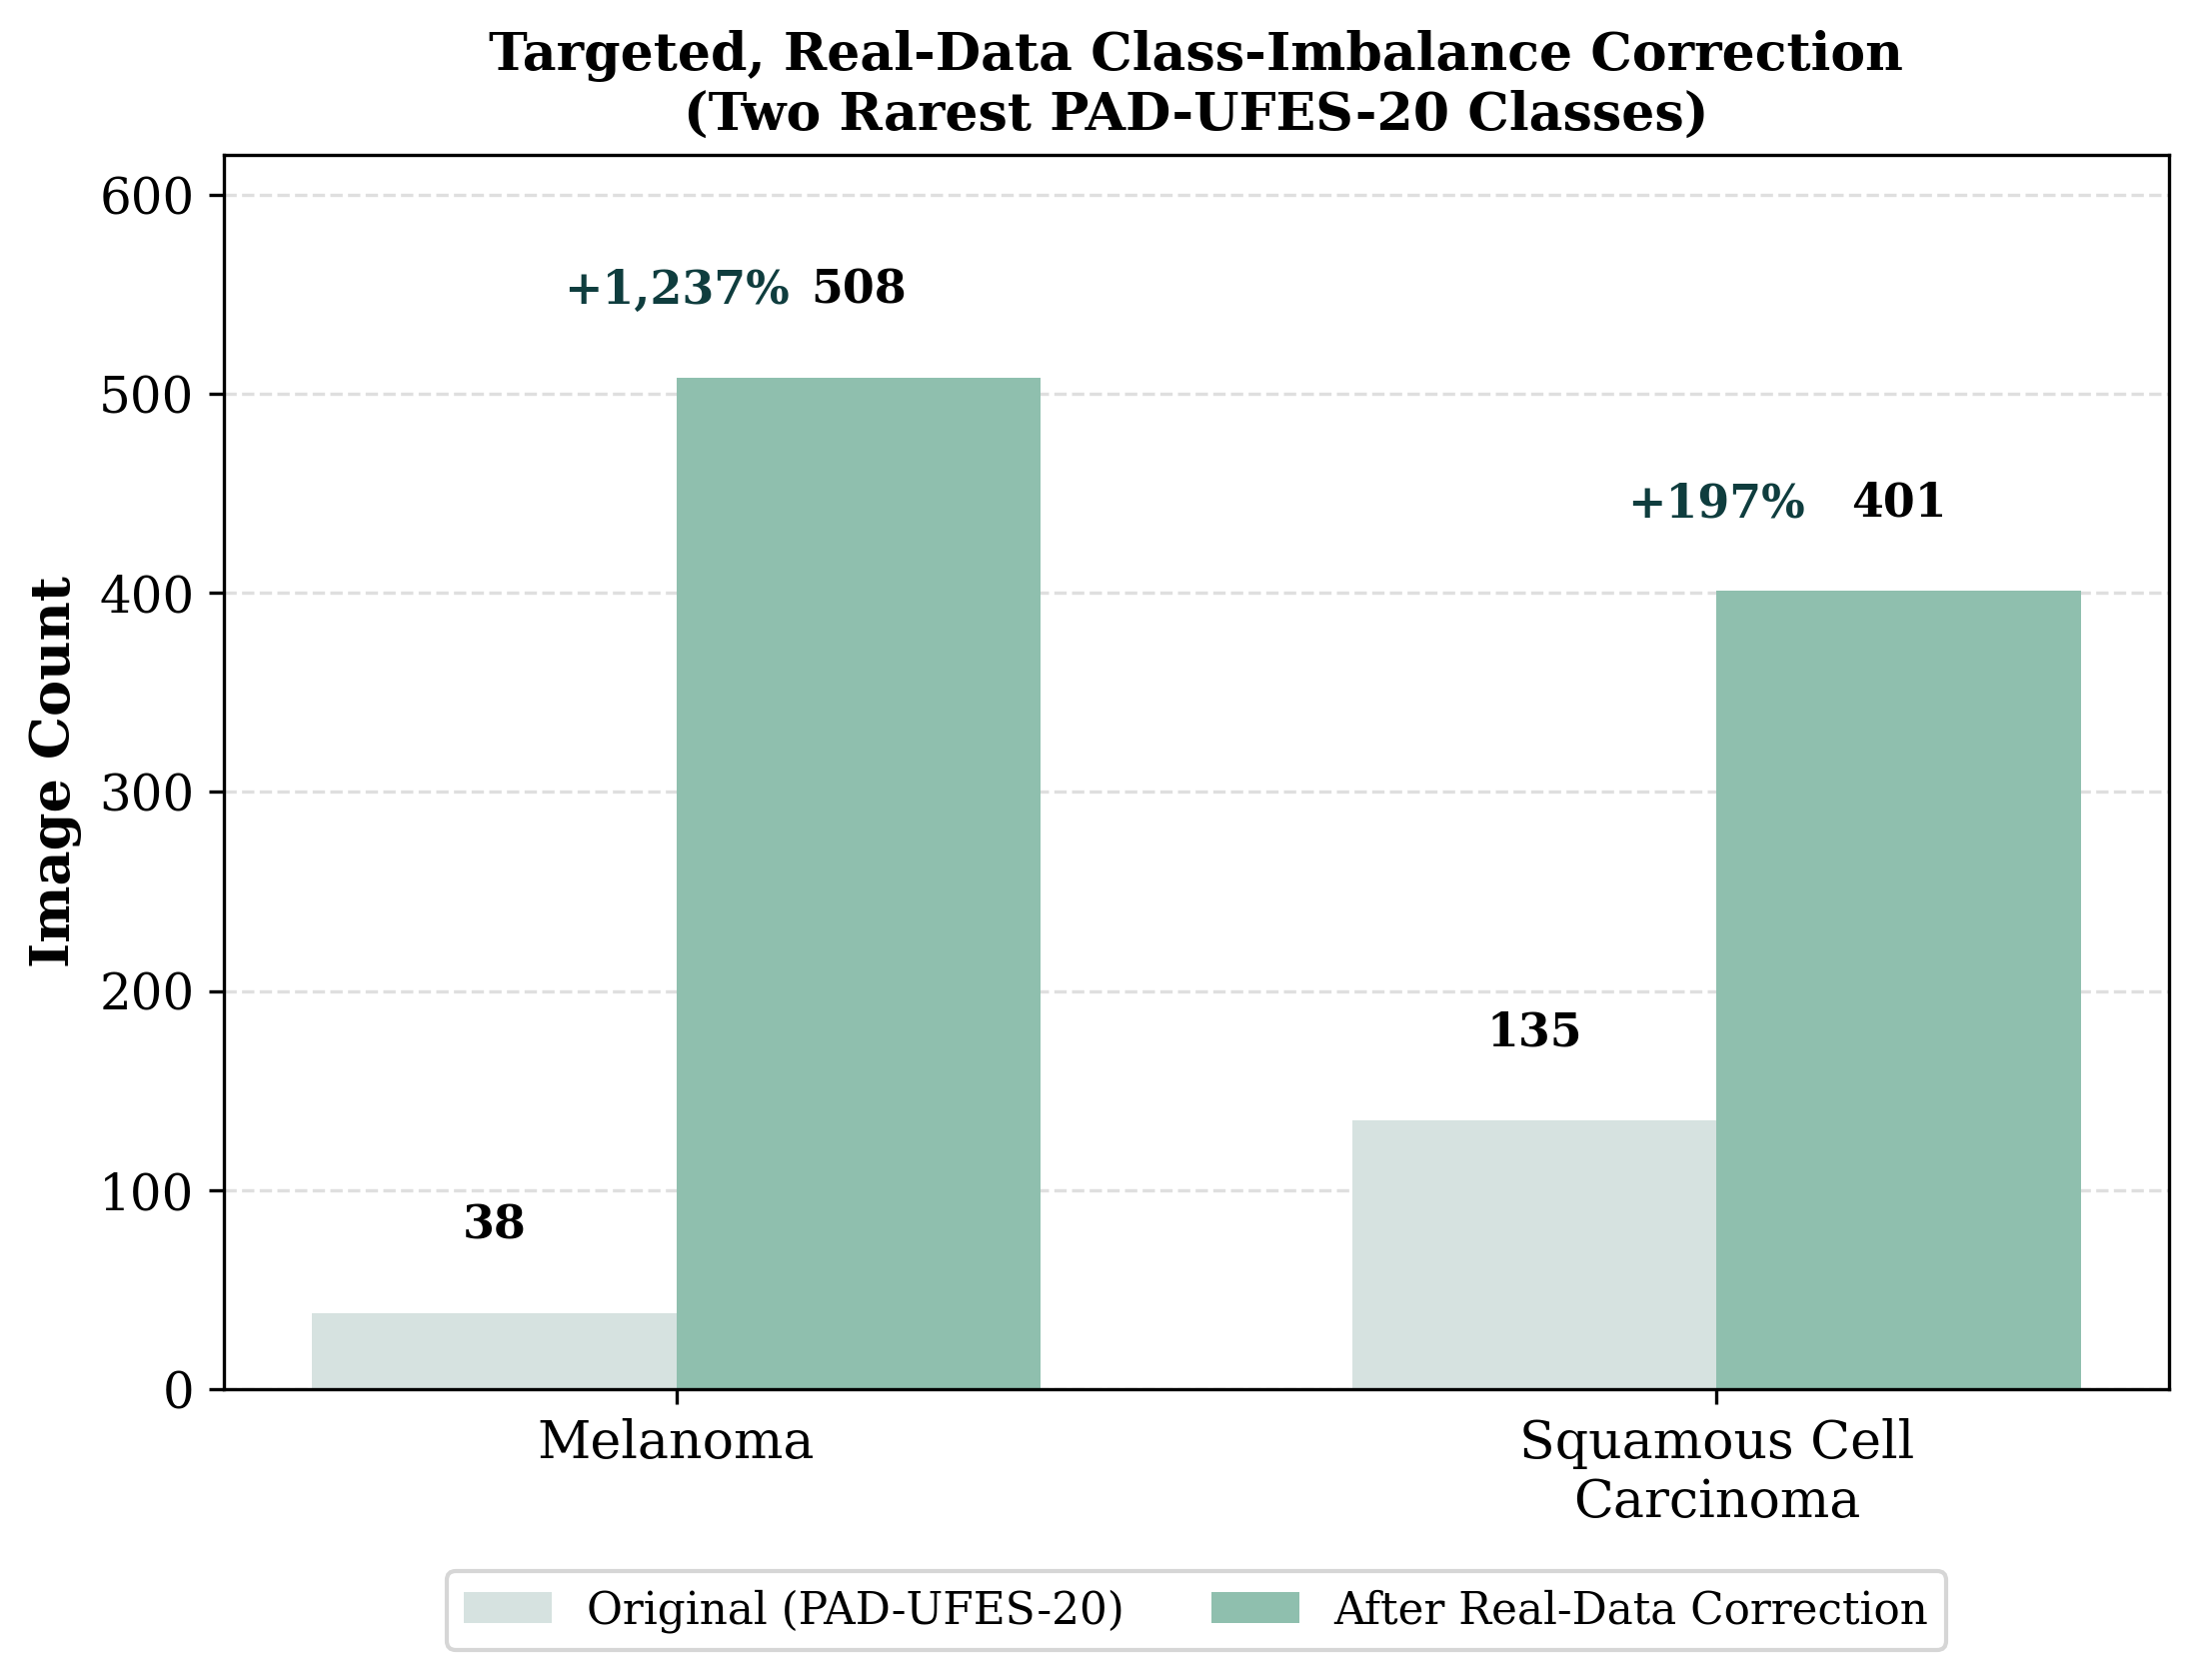
\includegraphics[width=0.85\columnwidth]{class_imbalance_correction.png}
\caption{Targeted, real-data class-imbalance correction for the two rarest PAD-UFES-20 classes, used only in later ablation experiments.}
\label{fig:imbalance}
\end{figure}

\subsection{Data Leakage Audit}
Prior to model development, every metadata column in each dataset was tested for statistical association with the diagnostic label using the phi coefficient and chi-square test. Columns exhibiting near-deterministic association with the label -- indicating that the field encodes post-diagnosis information rather than pre-diagnosis clinical observation -- were excluded. The most severe example was PAD-UFES-20's \texttt{biopsed} field, which was True in 100\% of malignant cases (phi = 0.80), reflecting the clinical practice of biopsying only lesions already suspected malignant. This audit identified and excluded twenty-two columns across the four datasets, yielding a documented feature whitelist per dataset (twenty-one features for PAD-UFES-20).

\subsection{Data Splitting}
All splits were performed at the patient level, never at the image level, to prevent images from the same individual appearing in both training and evaluation partitions. PAD-UFES-20 was split 70/15/15 with a fixed seed (42) for reproducibility. The test partition was evaluated under a single-use guard mechanism that raises an error on any repeated access.

\subsection{Proposed Hierarchical Architecture}
Figure \ref{fig:arch} details our proposed hierarchical architecture as a nine-stage pipeline. The image branch is an EfficientNet-B0 convolutional network, initialized with ImageNet-pretrained weights and fully fine-tuned; its pre-pooling feature map yields forty-nine spatial tokens. The metadata branch is a multilayer perceptron mapping an 89-dimensional (one-hot encoded) clinical feature vector to a 64-dimensional embedding. Before cross-attention, a metadata-conditioned channel gate (MetadataChannelGate) modulates the 49 image tokens: a sigmoid function of the metadata embedding produces a 1280-dimensional gate applied uniformly across all spatial tokens' channels, allowing clinical context to influence low-level image features prior to the attention-based fusion step. Both raw representations are then projected into a shared 256-dimensional space: the gated image tokens through a Key/Value projection, metadata through a Query projection. An 8-head cross-attention module then fuses them -- the metadata Query attends over the image Key/Value tokens, producing a 256-dimensional attended vector. This is concatenated with the original 64-dimensional metadata embedding into a 320-dimensional joint representation, which is passed through a classification head (FC $\to$ BatchNorm $\to$ ReLU $\to$ Dropout $\to$ FC(6)) to produce the final six-class prediction. Both branches are warm-started from independently pretrained single-modality checkpoints and subsequently fine-tuned end-to-end.

\begin{figure}[t]
\centering
\includegraphics[width=0.85\columnwidth]{Architecture_Diagram.pdf}
\caption{Proposed hierarchical cross-attention fusion architecture. Image tokens pass through a metadata-conditioned channel gate before image and metadata paths are projected into a shared 256-dimensional space, fused via an 8-head cross-attention block (Q=metadata, K=V=gated image tokens), and classified through a joint head.}
\label{fig:arch}
\end{figure}

We selected cross-attention over simple feature concatenation (late fusion) because the latter suffers from a dimensional imbalance: a 1,280-dimensional image embedding numerically dominates a 64-dimensional metadata embedding when directly concatenated, causing the fused representation to be driven almost entirely by the image modality. Projecting both modalities into a shared attention space before fusion avoids this imbalance, and allows the model to learn which spatial regions of the lesion are most relevant given a specific patient's clinical profile.

\subsection{Training Configuration}
All models were trained with the Adam optimizer, class-weighted cross-entropy loss, three random seeds per configuration, and early stopping (patience of seven epochs) based on validation macro-F1.

\section{Experiments and Results}

\subsection{Primary Results}
Table \ref{tab:primary} reports validation and test macro-F1 for the four primary model variants on PAD-UFES-20. The cross-attention fusion model achieves the best performance on both partitions, with a test macro-F1 of 0.6977, a 9-percentage-point improvement over the metadata-only baseline. The same test predictions also give a mean accuracy of 0.763; we report macro-F1 as the headline metric throughout, since it weights all six classes equally, whereas accuracy is dominated by the majority classes.

\begin{table}[t]
\caption{Primary results on PAD-UFES-20 (macro-F1, mean over 3 seeds)}
\label{tab:primary}
\centering
\begin{tabular}{|l|c|c|}
\hline
\textbf{Model} & \textbf{Validation} & \textbf{Test} \\
\hline
Image-only & 0.5703 $\pm$ 0.0130 & 0.6175 $\pm$ 0.0153 \\
\hline
Metadata-only & 0.5762 $\pm$ 0.0072 & 0.6077 $\pm$ 0.0202 \\
\hline
Late Fusion & 0.5731 $\pm$ 0.0021 & 0.6566 $\pm$ 0.0234 \\
\hline
\textbf{Cross-Attention} & \textbf{0.6209 $\pm$ 0.0143} & \textbf{0.6977 $\pm$ 0.0269} \\
\hline
\end{tabular}
\\[2pt]
\raggedright{\scriptsize Paired bootstrap (1,000 resamples): cross-attention's test-set gain is significant vs. every baseline -- image $p<0.001$, metadata $p=0.006$, late fusion $p=0.002$ (all significant under Bonferroni-corrected $\alpha=0.0167$).}
\end{table}

Table \ref{tab:confmat} shows the test-set confusion matrix (summed over 3 seeds, 1,062 predictions). The dominant error cluster is among Actinic Keratosis (AK), Basal Cell Carcinoma (BCC), and Squamous Cell Carcinoma (SCC) -- three keratinocyte-lineage, actinic-damage-spectrum classes that account for 172 of 252 total misclassifications (68.3\%), with SCC$\to$BCC (51 cases) the single largest confusion. This corroborates Pacheco and Krohling's (2020) clinical finding that these classes remain difficult to separate even with metadata available. Per-class performance mirrors this pattern: Actinic Keratosis reaches F1 = 0.83 (precision 0.85, recall 0.82) and Basal Cell Carcinoma F1 = 0.81 (precision 0.79, recall 0.82), while Melanoma reaches F1 = 0.73 (precision 0.80, recall 0.67) despite only 24 test instances, and Squamous Cell Carcinoma -- the class most entangled with BCC -- is the weakest at F1 = 0.25 (precision 0.29, recall 0.23), consistent with its severe test-set scarcity (32 images) and motivating the targeted class-imbalance correction in Section III-A.

\begin{table}[t]
\caption{Confusion matrix, cross-attention model, PAD-UFES-20 test (summed, 3 seeds)}
\label{tab:confmat}
\centering
\scriptsize
\begin{tabular}{|l|c|c|c|c|c|c|}
\hline
& \textbf{AK} & \textbf{BCC} & \textbf{MEL} & \textbf{NEV} & \textbf{SEK} & \textbf{SCC} \\
\hline
\textbf{AK} & \cellcolor{diagcolor!60}268 & \cellcolor{offdiagcolor!14}22 & 0 & 0 & \cellcolor{offdiagcolor!13}17 & \cellcolor{offdiagcolor!13}20 \\
\hline
\textbf{BCC} & \cellcolor{offdiagcolor!15}30 & \cellcolor{diagcolor!70}328 & 0 & \cellcolor{offdiagcolor!11}4 & \cellcolor{offdiagcolor!10}3 & \cellcolor{offdiagcolor!16}34 \\
\hline
\textbf{MEL} & 0 & 0 & \cellcolor{diagcolor!18}16 & \cellcolor{offdiagcolor!11}8 & 0 & 0 \\
\hline
\textbf{NEV} & \cellcolor{offdiagcolor!10}1 & \cellcolor{offdiagcolor!11}8 & \cellcolor{offdiagcolor!10}1 & \cellcolor{diagcolor!29}87 & \cellcolor{offdiagcolor!11}8 & 0 \\
\hline
\textbf{SEK} & \cellcolor{offdiagcolor!10}3 & \cellcolor{offdiagcolor!11}4 & \cellcolor{offdiagcolor!10}2 & \cellcolor{offdiagcolor!12}12 & \cellcolor{diagcolor!30}89 & \cellcolor{offdiagcolor!10}1 \\
\hline
\textbf{SCC} & \cellcolor{offdiagcolor!12}15 & \cellcolor{offdiagcolor!18}51 & \cellcolor{offdiagcolor!10}1 & 0 & \cellcolor{offdiagcolor!11}7 & \cellcolor{diagcolor!19}22 \\
\hline
\end{tabular}
\end{table}

\begin{table}[t]
\caption{Per-class precision, recall, and F1 (cross-attention model, summed 3 seeds)}
\label{tab:perclass}
\centering
\begin{tabular}{|l|c|c|c|c|}
\hline
\textbf{Class} & \textbf{Support} & \textbf{Precision} & \textbf{Recall} & \textbf{F1} \\
\hline
AK & 327 & 0.8454 & 0.8196 & 0.8323 \\
\hline
BCC & 399 & 0.7942 & 0.8221 & 0.8079 \\
\hline
MEL & 24 & 0.8000 & 0.6667 & 0.7273 \\
\hline
NEV & 105 & 0.7838 & 0.8286 & 0.8056 \\
\hline
SEK & 111 & 0.7177 & 0.8018 & 0.7574 \\
\hline
SCC & 96 & 0.2857 & 0.2292 & 0.2543 \\
\hline
\textbf{Macro avg} & 1062 & 0.7045 & 0.6947 & 0.6975 \\
\hline
\end{tabular}
\end{table}

\subsection{Cross-Dataset Generalization}
We evaluated PAD-UFES-20-trained models on HAM10000's three shared diagnostic classes (Basal Cell Carcinoma, Melanoma, Nevus). Table \ref{tab:crossdataset} reports the resulting macro-F1 scores. Cross-attention fusion (0.4654) is not statistically distinguishable from image-only (0.4658, bootstrap $p=0.970$) or late fusion (0.4597, $p=0.590$), but significantly outperforms metadata-only (0.2920, $p<0.001$) -- reflecting HAM10000's substantially sparser metadata schema. We report this honestly: cross-attention demonstrably wins the modality-value question but does not yet demonstrate superior pure generalization relative to image-only features.

\begin{table}[t]
\caption{PAD-UFES-20 $\rightarrow$ HAM10000 cross-dataset macro-F1}
\label{tab:crossdataset}
\centering
\begin{tabular}{|l|c|}
\hline
\textbf{Model} & \textbf{Macro-F1} \\
\hline
Image-only & 0.4658 $\pm$ 0.0373 \\
\hline
Metadata-only & 0.2920 $\pm$ 0.0121 \\
\hline
Late Fusion & 0.4597 $\pm$ 0.0084 \\
\hline
Cross-Attention Fusion & 0.4654 $\pm$ 0.0197 \\
\hline
\end{tabular}
\end{table}

\subsection{External Validation and Fairness Analysis}
HAM10000-trained checkpoints were further evaluated on ISIC Archive 1 and Archive 2 without additional fine-tuning. Because HAM10000 shares substantial image provenance with both archives (98.6\% overlap with Archive 2, 66.5\% with Archive 1), overlapping images were identified and excluded from the evaluation sets via a dedicated exclusion list (1,362 IDs), so the reported numbers reflect genuinely unseen data. Image-only macro-F1 was 0.4912 $\pm$ 0.0094 on Archive 2 and 0.2421 $\pm$ 0.0118 on Archive 1 (the latter driven by near-zero support for two of five shared classes, not worse generalization). On Archive 2, image-only significantly outperformed metadata-only (0.2410 $\pm$ 0.0295; bootstrap diff +0.2502, 95\% CI [+0.2368, +0.2641], $p<0.001$), the largest, most statistically decisive effect in this study. A Fitzpatrick skin-tone fairness analysis on PAD-UFES-20's test partition found cross-attention fusion to be the best- or tied-best-performing model within every Fitzpatrick group with sufficient sample size for evaluation; however, the two darkest categories (Types V and VI) contained only two and one test images respectively, and 38\% of test records lacked a recorded Fitzpatrick value. We report this as a genuine data-availability limitation rather than a definitive fairness conclusion, consistent with Alipour et al.'s (2024) finding that skin-tone underrepresentation is systemic across public dermatology datasets.

\subsection{Extended Ablations}
Motivated by the observation that our reported macro-F1 is comparatively modest relative to some binary or accuracy-based literature results, we conducted four further, pre-registered ablations to determine whether performance could be meaningfully improved through legitimate architectural or data changes. Table \ref{tab:ablations} summarizes these results.

\begin{table}[t]
\caption{Extended ablation results (PAD-UFES-20)}
\label{tab:ablations}
\centering
\scriptsize
\begin{tabular}{|p{2.6cm}|p{1.9cm}|p{2.1cm}|}
\hline
\textbf{Experiment} & \textbf{Val. macro-F1} & \textbf{Outcome} \\
\hline
5-backbone comparison & 0.5859--0.6224 & All exceeded baseline \\
\hline
Dataset-expansion only & 0.6186 $\pm$ 0.0124 & $\approx$ baseline \\
\hline
Dual-backbone ensemble & 0.6856; 0.7321(test) & $p=0.062$, not sig. \\
\hline
Joint 3-way fusion & 0.6721 & Exceeded 0.6710 bar by only +0.0011, below clear-and-meaningful threshold \\
\hline
\end{tabular}
\end{table}

The dataset-expansion-only ablation isolates the effect of adding real, biopsy-confirmed Melanoma and Squamous Cell Carcinoma images (Figure \ref{fig:imbalance}) without changing the model architecture; its near-identical result to the original baseline indicates that the larger performance gains observed with backbone substitution are attributable primarily to architectural capacity and representation quality, not to training-set size alone -- despite the 1,237\% and 197\% class-size increases shown above. For the dual-backbone ensemble, we had pre-registered a decision rule prior to observing results: a third, final read of the held-out test set would only be authorized if a candidate model's validation score clearly and meaningfully exceeded the strongest single-backbone validation result (0.6710). The ensemble's validation mean (0.6856) satisfied this criterion and was granted a one-time test evaluation, yielding 0.7321; bootstrap testing against the original headline result, however, returned $p=0.062$, narrowly missing the conventional 0.05 significance threshold. The joint three-way fusion model's validation mean (0.6721) did not clearly exceed the same 0.6710 threshold and was therefore not granted a test evaluation, consistent with the pre-registered protocol. We report both outcomes transparently rather than selectively.

\section{Discussion}

\subsection{Interpretation of Results}
Several methodological choices explain why our reported scores are lower than some values reported elsewhere in the literature. First, we address a more difficult six-class problem rather than the common binary (malignant/benign) framing, and report macro-F1 rather than accuracy, which on imbalanced data can appear high even when a model performs poorly on minority classes, whereas macro-F1 weights every class equally. Second, our documented leakage audit removed twenty-two features that would otherwise have allowed shortcut learning. Restricted to studies using comparably rigorous multi-class, macro-F1-based evaluation, our result compares favorably. The confusion matrix (Table \ref{tab:confmat}) shows this is a genuine, clinically-explainable difficulty rather than an architectural weakness, since the confused classes share the same actinic-damage-spectrum lineage: a model that struggles on classes also difficult for clinicians to distinguish is behaving reasonably, whereas confusion among clinically dissimilar classes would instead point to a genuine modeling deficiency. Unlike the cross-dataset transfer comparisons (Section IV-C, all non-significant, $p \geq 0.59$) and the dual-backbone ensemble ($p=0.062$), the primary in-distribution comparison is the one result where cross-attention's advantage over every baseline is both numerically consistent and statistically robust (all $p \leq 0.006$, Bonferroni-corrected) -- the architecture's benefit is real within-distribution even though it does not yet translate into superior cross-dataset generalization.

The dataset-expansion-only ablation is a notable methodological finding in its own right: adding real, correctly-labeled training data for the weakest classes, without a corresponding architectural improvement, produced negligible gains, whereas substituting the image backbone alone produced substantial gains. This suggests that, for this problem and dataset scale, model capacity and inductive bias were a more binding constraint than raw training-set size -- with practical implications for future work prioritization in similarly-sized dermatology datasets.

The ensemble result (0.7321 test, $p=0.062$) illustrates a further methodological point. We observed a consistent pattern of validation-to-test score increases (the primary model: $+0.077$; the ensemble: $+0.047$), under which the joint fusion model's test score -- had it been evaluated -- might plausibly also have exceeded its validation score. We explicitly chose not to pursue this test evaluation, since doing so specifically because of a post-hoc ``it might do better'' expectation would undermine the purpose of pre-registering a decision threshold before observing results. We regard this as a disciplined limitation rather than an oversight.

We similarly rejected a separate ensemble-plus-test-time-augmentation (TTA) variant of the cross-attention model, evaluated independently of the dual-backbone ensemble above. Aggregate macro-F1 also regressed under this variant (0.6213 to 0.5886), but the more clinically decisive finding came from per-class inspection: Melanoma F1 collapsed from 0.3636 to 0.20 -- the rarest, highest-stakes class in this task. We treat this per-class collapse, not the aggregate drop alone, as disqualifying on clinical-relevance grounds, reflecting this work's broader emphasis on per-class and statistically-grounded validation over headline-number optimization.

\subsection{Limitations}
This study has several limitations that should inform how its results are interpreted. First, our fairness analysis is constrained by severe sample-size imbalance across Fitzpatrick skin-tone categories in PAD-UFES-20, particularly Types V and VI; findings should be read as suggestive rather than statistically conclusive for the darkest skin tones. Second, our cross-dataset evaluation is limited to three diagnostic classes shared between PAD-UFES-20 and HAM10000, since the two datasets do not share an identical taxonomy. Third, the dual-backbone ensemble and joint three-way fusion results, while promising, remain unconfirmed on a genuinely independent test set under our pre-registered protocol. Finally, all datasets originate from a small number of geographic and clinical contexts, and further external validation across more diverse populations and imaging equipment would strengthen real-world generalizability claims. We also did not profile inference latency or memory footprint; the extended two-backbone variants (Section IV-E) roughly double image-branch computation relative to the primary model, and a full deployment-readiness assessment is left to future work.

\section{Conclusion and Future Work}
We presented a metadata-guided cross-attention fusion architecture for multimodal skin lesion classification, achieving 0.6977 test macro-F1 on PAD-UFES-20 under a six-class, leakage-audited, patient-wise-split protocol. Beyond the primary result, we contribute a transparent, pre-registered methodology for extended architectural and data ablations, cross-dataset generalization testing, statistical significance testing, and skin-tone fairness analysis -- demonstrating that methodological rigor and honest reporting of both positive and inconclusive findings are essential complements to raw predictive accuracy in clinically-oriented dermatology AI. Multimodal fusion substantially improves controlled, in-distribution performance, but rigorous cross-dataset evaluation reveals this does not automatically translate into domain robustness -- underscoring that evaluation methodology matters as much as architecture.

Several directions follow directly from our findings. First, a fresh, independently-held-out evaluation set would allow the dual-backbone ensemble and joint three-way fusion results to be legitimately re-tested without compromising our current pre-registered protocol. Second, since the confusion matrix identifies Actinic Keratosis, Basal Cell Carcinoma, and Squamous Cell Carcinoma as a persistent, clinically-explainable error cluster, targeted data collection or a dedicated sub-classifier for this keratinocyte-lineage group is promising. Third, a multi-institution collaboration to collect labeled images across the full Fitzpatrick spectrum would enable a more statistically powered fairness evaluation, potentially using equalized-odds metrics beyond the per-group macro-F1 reported here. Finally, lesion segmentation as a pre-processing step, deferred here to avoid confounding it with the ablations already in progress, remains a reasoned, sequenced direction for isolating any further gains it may offer.

\section*{Reproducibility Statement}
All datasets used are publicly available under their respective original licenses and were de-identified by their publishers prior to release; no additional patient contact or identification was performed by the authors. Full hyperparameter details beyond Section III are available from the authors upon request.

\section*{Acknowledgment}
The authors thank the creators of PAD-UFES-20, HAM10000, and the ISIC Archive for making their datasets publicly available, enabling this study's cross-dataset and external validation experiments.

\footnotesize
\begin{thebibliography}{00}
\bibitem{pacheco2020} A. G. C. Pacheco et al., ``PAD-UFES-20: A skin lesion dataset composed of patient data and clinical images collected from smartphones,'' \emph{Data in Brief}, vol. 32, 2020.
\bibitem{tschandl2018} P. Tschandl, C. Rosendahl, and H. Kittler, ``The HAM10000 dataset,'' \emph{Scientific Data}, vol. 5, 2018.
\bibitem{trace2024} D. Christopoulos, S. Spanos, V. Ntouskos, and K. Karantzalos, ``TRACE: Transformer-based Risk Assessment for Clinical Evaluation,'' arXiv:2411.08701, 2024.
\bibitem{shrestha2026} A. Shrestha and A. Palit, ``Multimodal skin disease classification using vision transformers, medical captioning, and metadata fusion: an analysis on the ISIC 2024 dataset,'' \emph{Biomedical Physics \& Engineering Express}, vol. 12, no. 2, art. 025043, 2026, DOI: 10.1088/2057-1976/ae4eeb.
\bibitem{pacheco2021} A. G. C. Pacheco and R. A. Krohling, ``An attention-based mechanism to combine images and metadata,'' \emph{IEEE JBHI}, 2021.
\bibitem{pacheco2020clinical} A. G. C. Pacheco and R. A. Krohling, ``The impact of patient clinical information on automated skin cancer detection,'' \emph{Computers in Biology and Medicine}, vol. 116, art. 103545, 2020.
\bibitem{daneshjou2022} R. Daneshjou et al., ``Disparities in dermatology AI performance,'' \emph{Science Advances}, vol. 8, no. 32, 2022.
\bibitem{alipour2024} N. Alipour et al., ``Diversity in skin lesion datasets: A review,'' \emph{Current Dermatology Reports}, 2024.
\end{thebibliography}

\vspace{-0pt}
\end{document}